\documentclass{article}

% Language setting
% Replace `english' with e.g. `spanish' to change the document language
\usepackage[english]{babel}

% Set page size and margins
% Replace `letterpaper' with `a4paper' for UK/EU standard size
\usepackage[letterpaper,top=2cm,bottom=2cm,left=3cm,right=3cm,marginparwidth=1.75cm]{geometry}

% Useful packages
\usepackage{amsmath}
\usepackage{graphicx}
\usepackage[colorlinks=true, allcolors=blue]{hyperref}
\usepackage{authblk}

\title{MVAR: A Mouse Variation Registry}
\author[1]{Bah\'{a} El Kassaby}
\author[1]{Francisco Castellanos}
\author[1]{Govindarajan Kunde-Ramamoorthy}
\author[1]{Carol Bult}
\affil[1]{The Jackson Laboratory, Bar Harbor, Maine, USA}

\begin{document}
\maketitle

\begin{abstract}
The Mouse Variation Registry (MVAR) project includes the implementation of a scalable database of unique mouse variations and their annotations, the development of data acquisition tools for variant data from multiple resources and the implementation of user interfaces for searching and displaying results.
\end{abstract}

\section{Background}

Model organisms are essential to understanding the biological and disease consequences of human genome variation. Bioinformatics resources that support meaningful comparisons of mouse and human genotype-to-phenotype data and knowledge are needed to support the translation from bench to bedside and back again \cite{manolio17}.

There is no genome variation resource for mouse comparable to resources available for human genome variation data such as EXAC \cite{karczewski17}, ClinVar \cite{landrum14}, or ClinGen \cite{rehm15}. NCBI resources such as dbSNP and ClinVar no longer accept data from model organisms. While the European Variation Archive (EVA) at the European Bioinformatics Institute (EBI) serves a repository of SNP data for mouse, however, the resource does not accept imputed variation data or curated phenotype annotations associated with variation data that are central to data interpretation and analysis. Although the Mouse Genome Informatics database (MGI) \cite{bult18} serves as a comprehensive mouse allele registry and curates information about the association of mouse variants with phenotypes and disease, the variation data in MGI are not currently available in format consistent with the Human Genome Variation Society (HGVS) standards \cite{hgvs}. The Mouse Variation Registry (MVAR) will represent the integration of all mouse genome variation data and includes processes to automatically canonicalize variants so that variants are uniquely represented in the database with comprehensive annotation and their distribution across strains.

\section{Source data}

The starting dataset used as input into MVAR was downloaded in VCF format \cite{vcf} (as a 42GB gzipped file) from the Mouse Genomes Project at the Wellcome-Sanger Institute \cite{mgp} and contains about 81M Single-Nucleotide Variants (SNV), ~9M Deletions and ~8M Insertions (See Figures \ref{fig:var_distrib}, \ref{fig:var_class}). Other data will be obtained from MGI, the Mouse Mutant Repository database (MMRDB), the Diversity Outbred Database (DODB), and from computationally imputed SNP data.

\begin{figure}
\centering
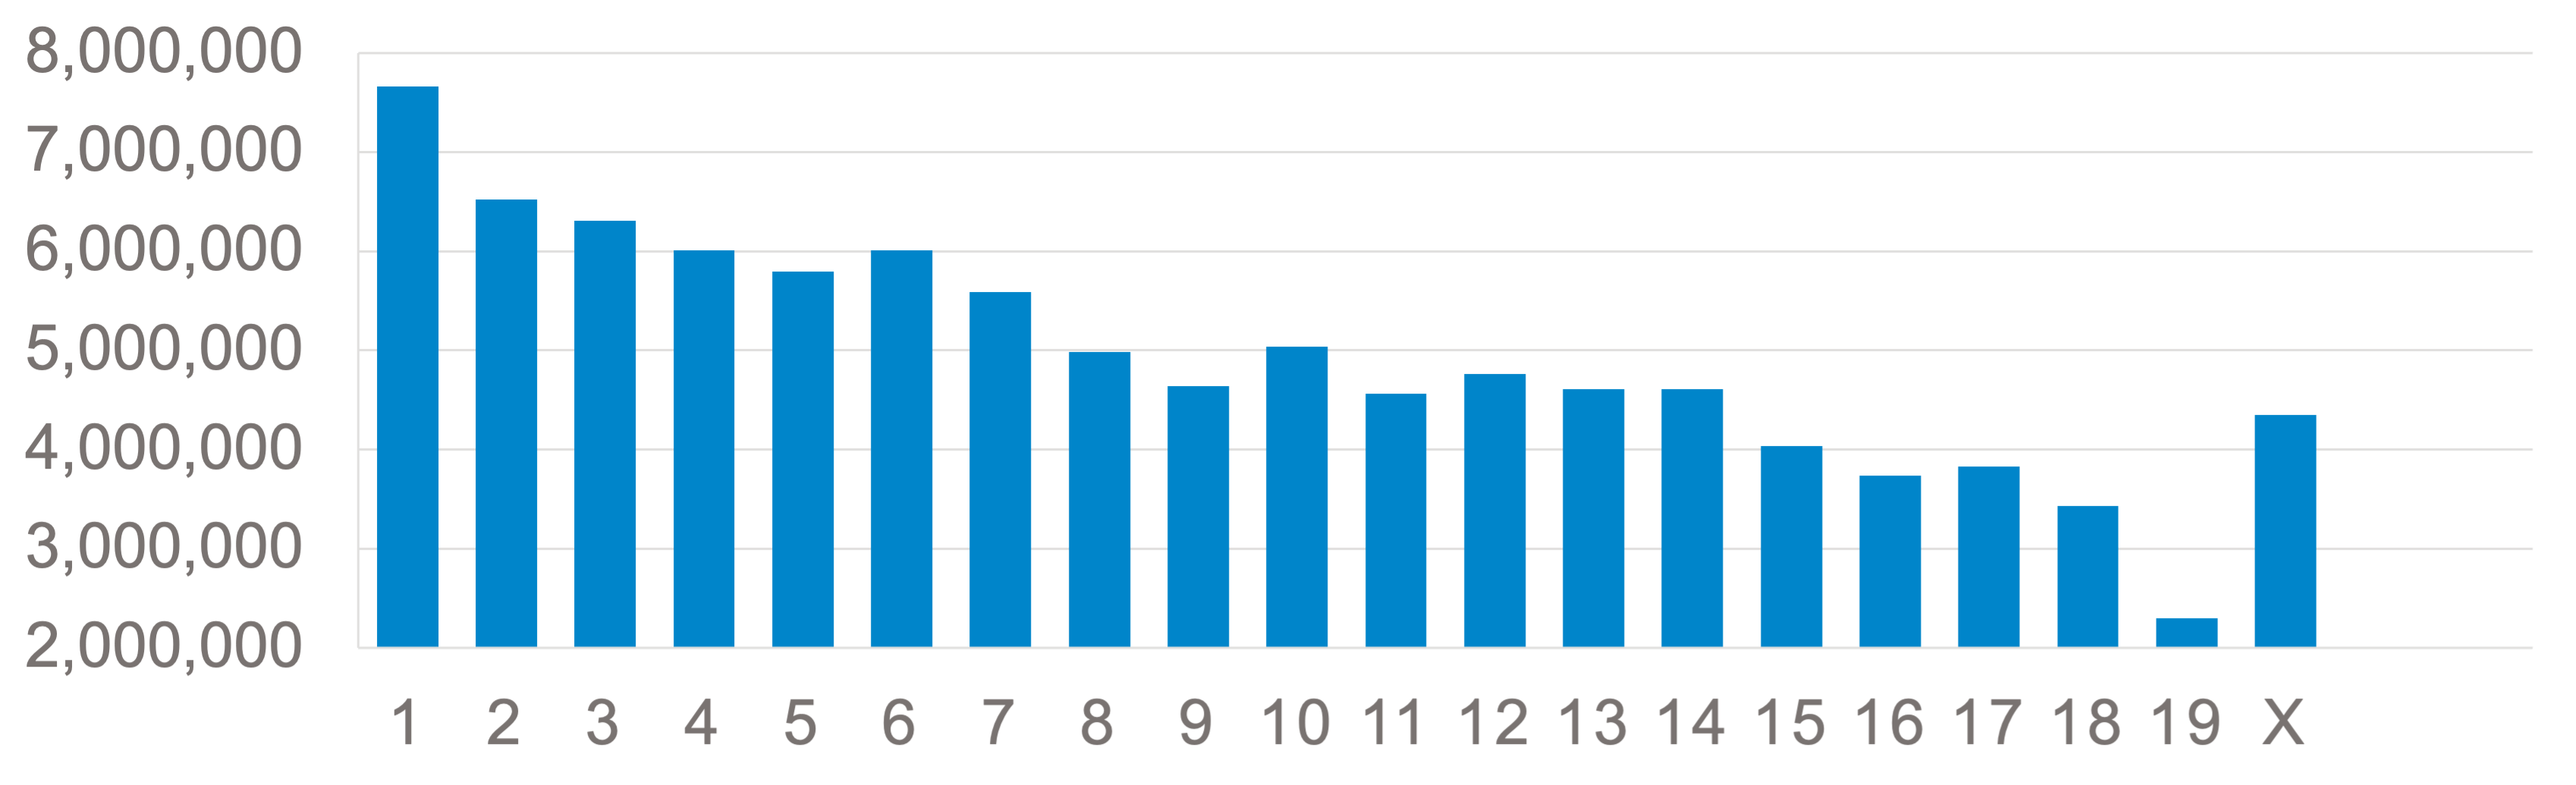
\includegraphics[width=0.75\linewidth]{var_distrib_rel_2005.png}
\caption{\label{fig:var_distrib}Variant distribution across chromosomes for Sanger REL 2005}
\end{figure}

\begin{figure}
\centering
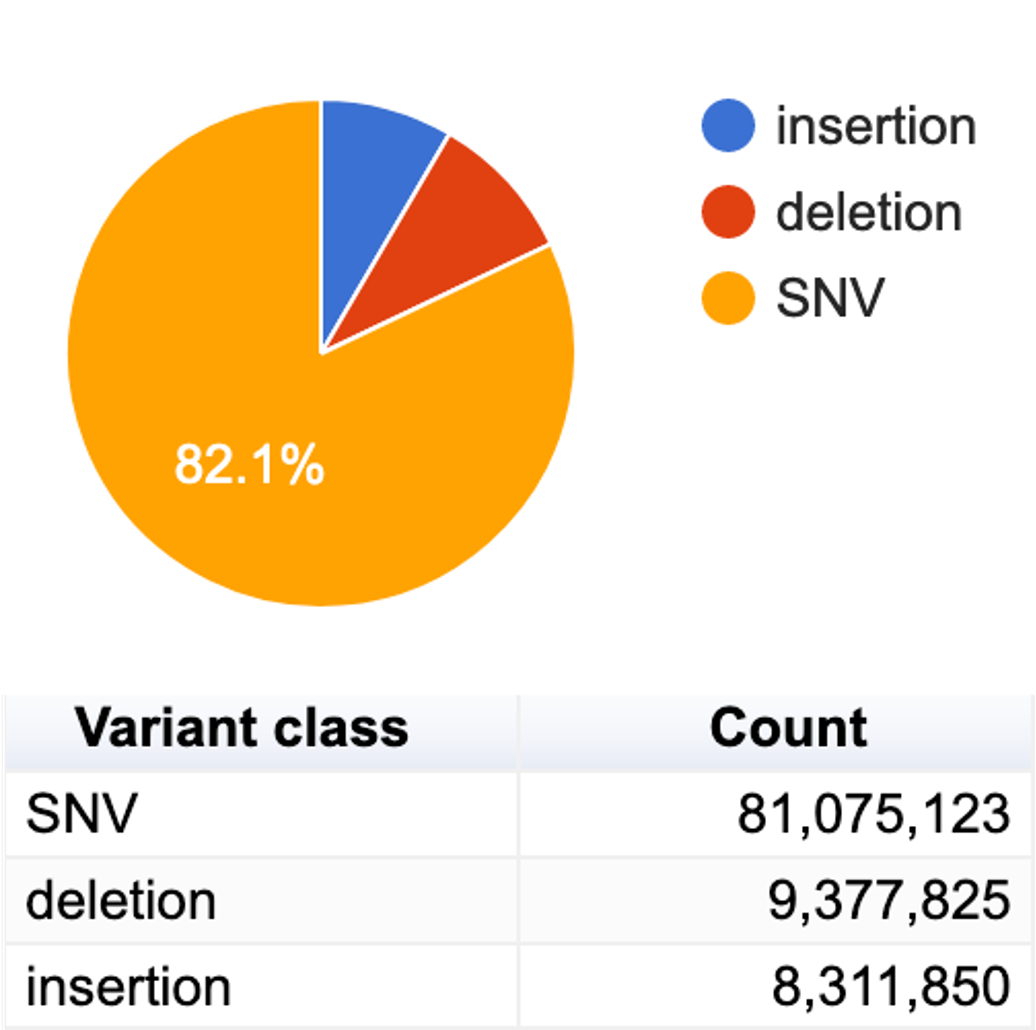
\includegraphics[width=0.5\linewidth]{var_class_rel_2005.png}
\caption{\label{fig:var_class}Variant Classes from Sanger REL 2005}
\end{figure}

\subsection{MM11/GRCm39}

Add paragraph about DB upgrade to mm11.


\section{MVAR data ingest workflow}

The MVAR data ingest workflow (See Figures \ref{fig:arch_diagram}, \ref{fig:pipeline}) has been developed to normalize, prepare and annotate input variation data. The normalization step of the pipeline consists of left aligning each variant i.e., shifting the start position of that variant to the left until it is no longer possible to do so. This is done using the GATK framework developed by the Broad Institute \cite{mckenna10}. During that process, the multi-allelic variants (where there is more than one variation in a row) are decomposed so that we end up with a variant per row. The next step in the pipeline is made with the use of the Ensembl Variant Effect Predictor (VEP) \cite{mclaren15}, which annotates the variation data with its corresponding HGVS nomenclature and existing external Id. The final step uses the Jannovar library \cite{jäger14} to enrich the data with Functional Consequence annotations. 

\begin{figure}
\centering
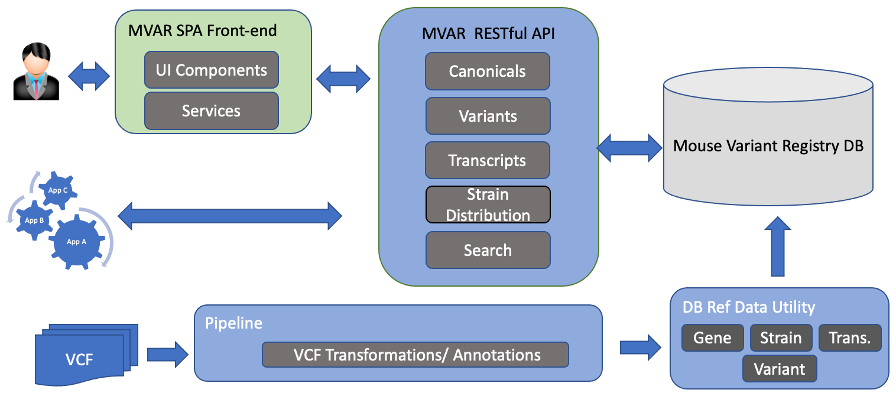
\includegraphics[width=0.8\linewidth]{architecture_diagram.png}
\caption{\label{fig:arch_diagram}Architecture diagram}
\end{figure}

\begin{figure}
\centering
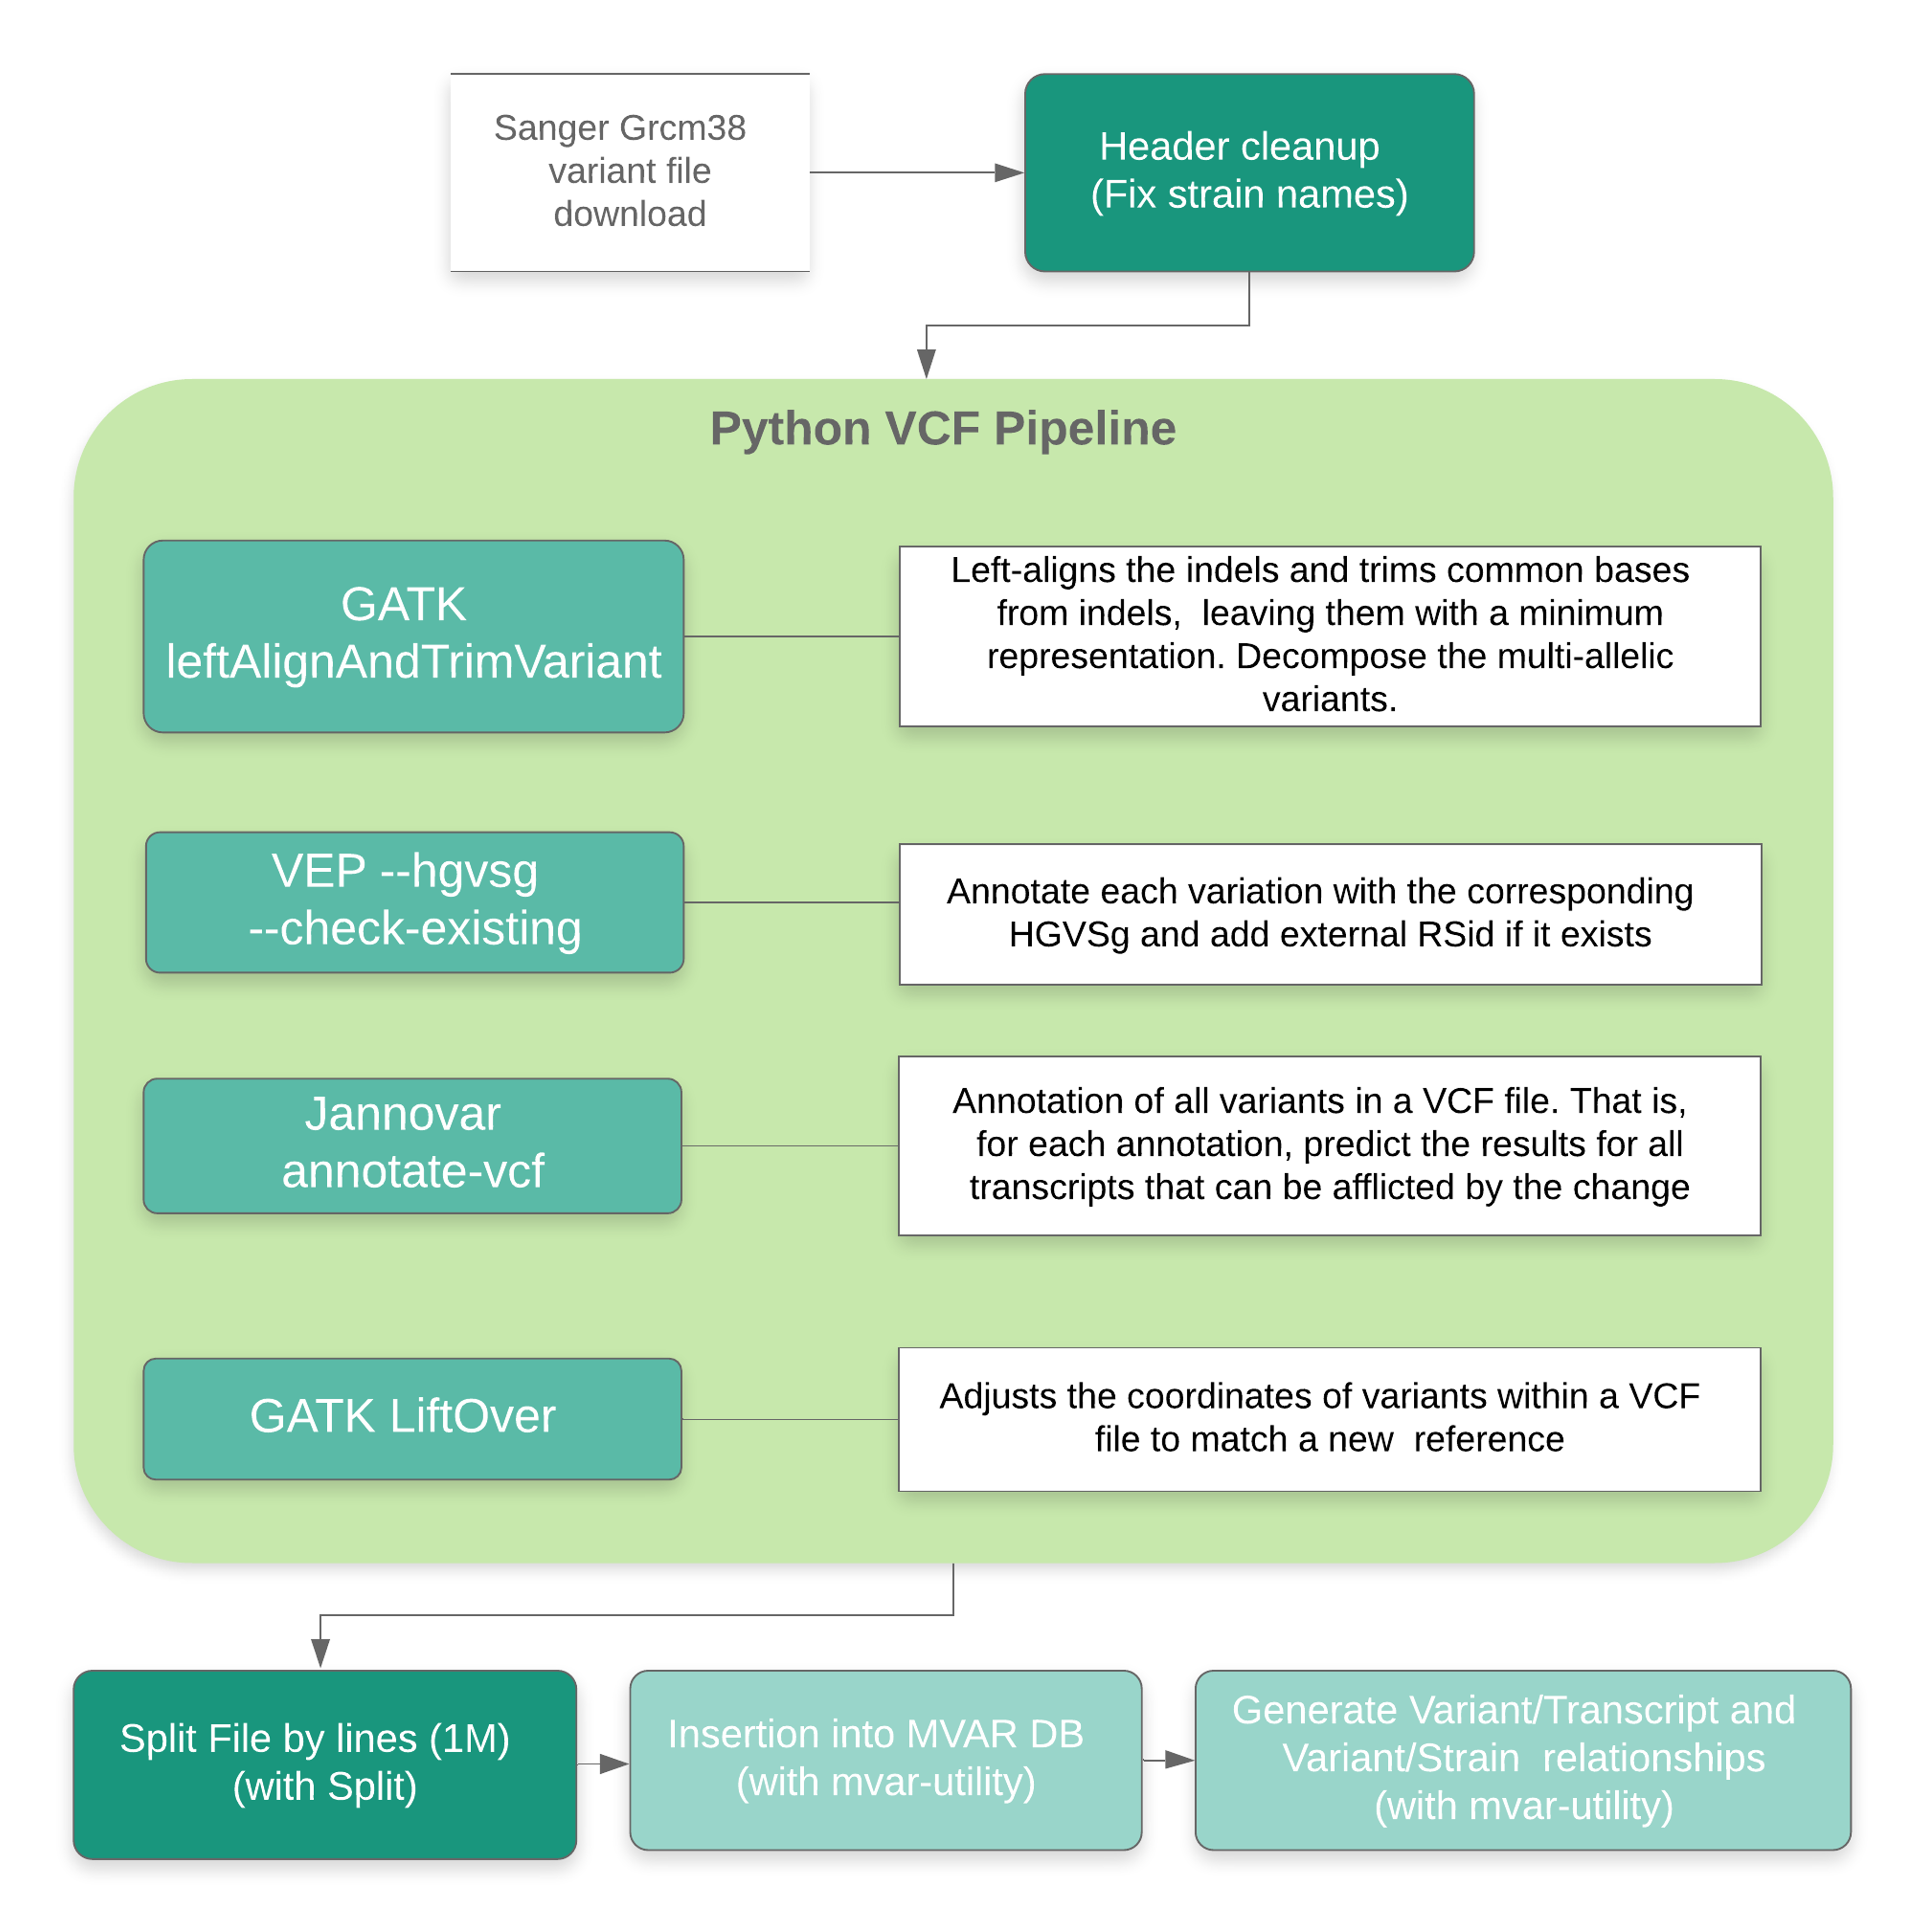
\includegraphics[width=0.8\linewidth]{pipeline.png}
\caption{\label{fig:pipeline}Data processing pipeline}
\end{figure}

After the data has been pre-processed through the pipeline, they are inserted into a MySQL database with the help of custom tools developed to create the canonical variants representations (See Figure \ref{fig:server_architecture}).

\begin{figure}
\centering
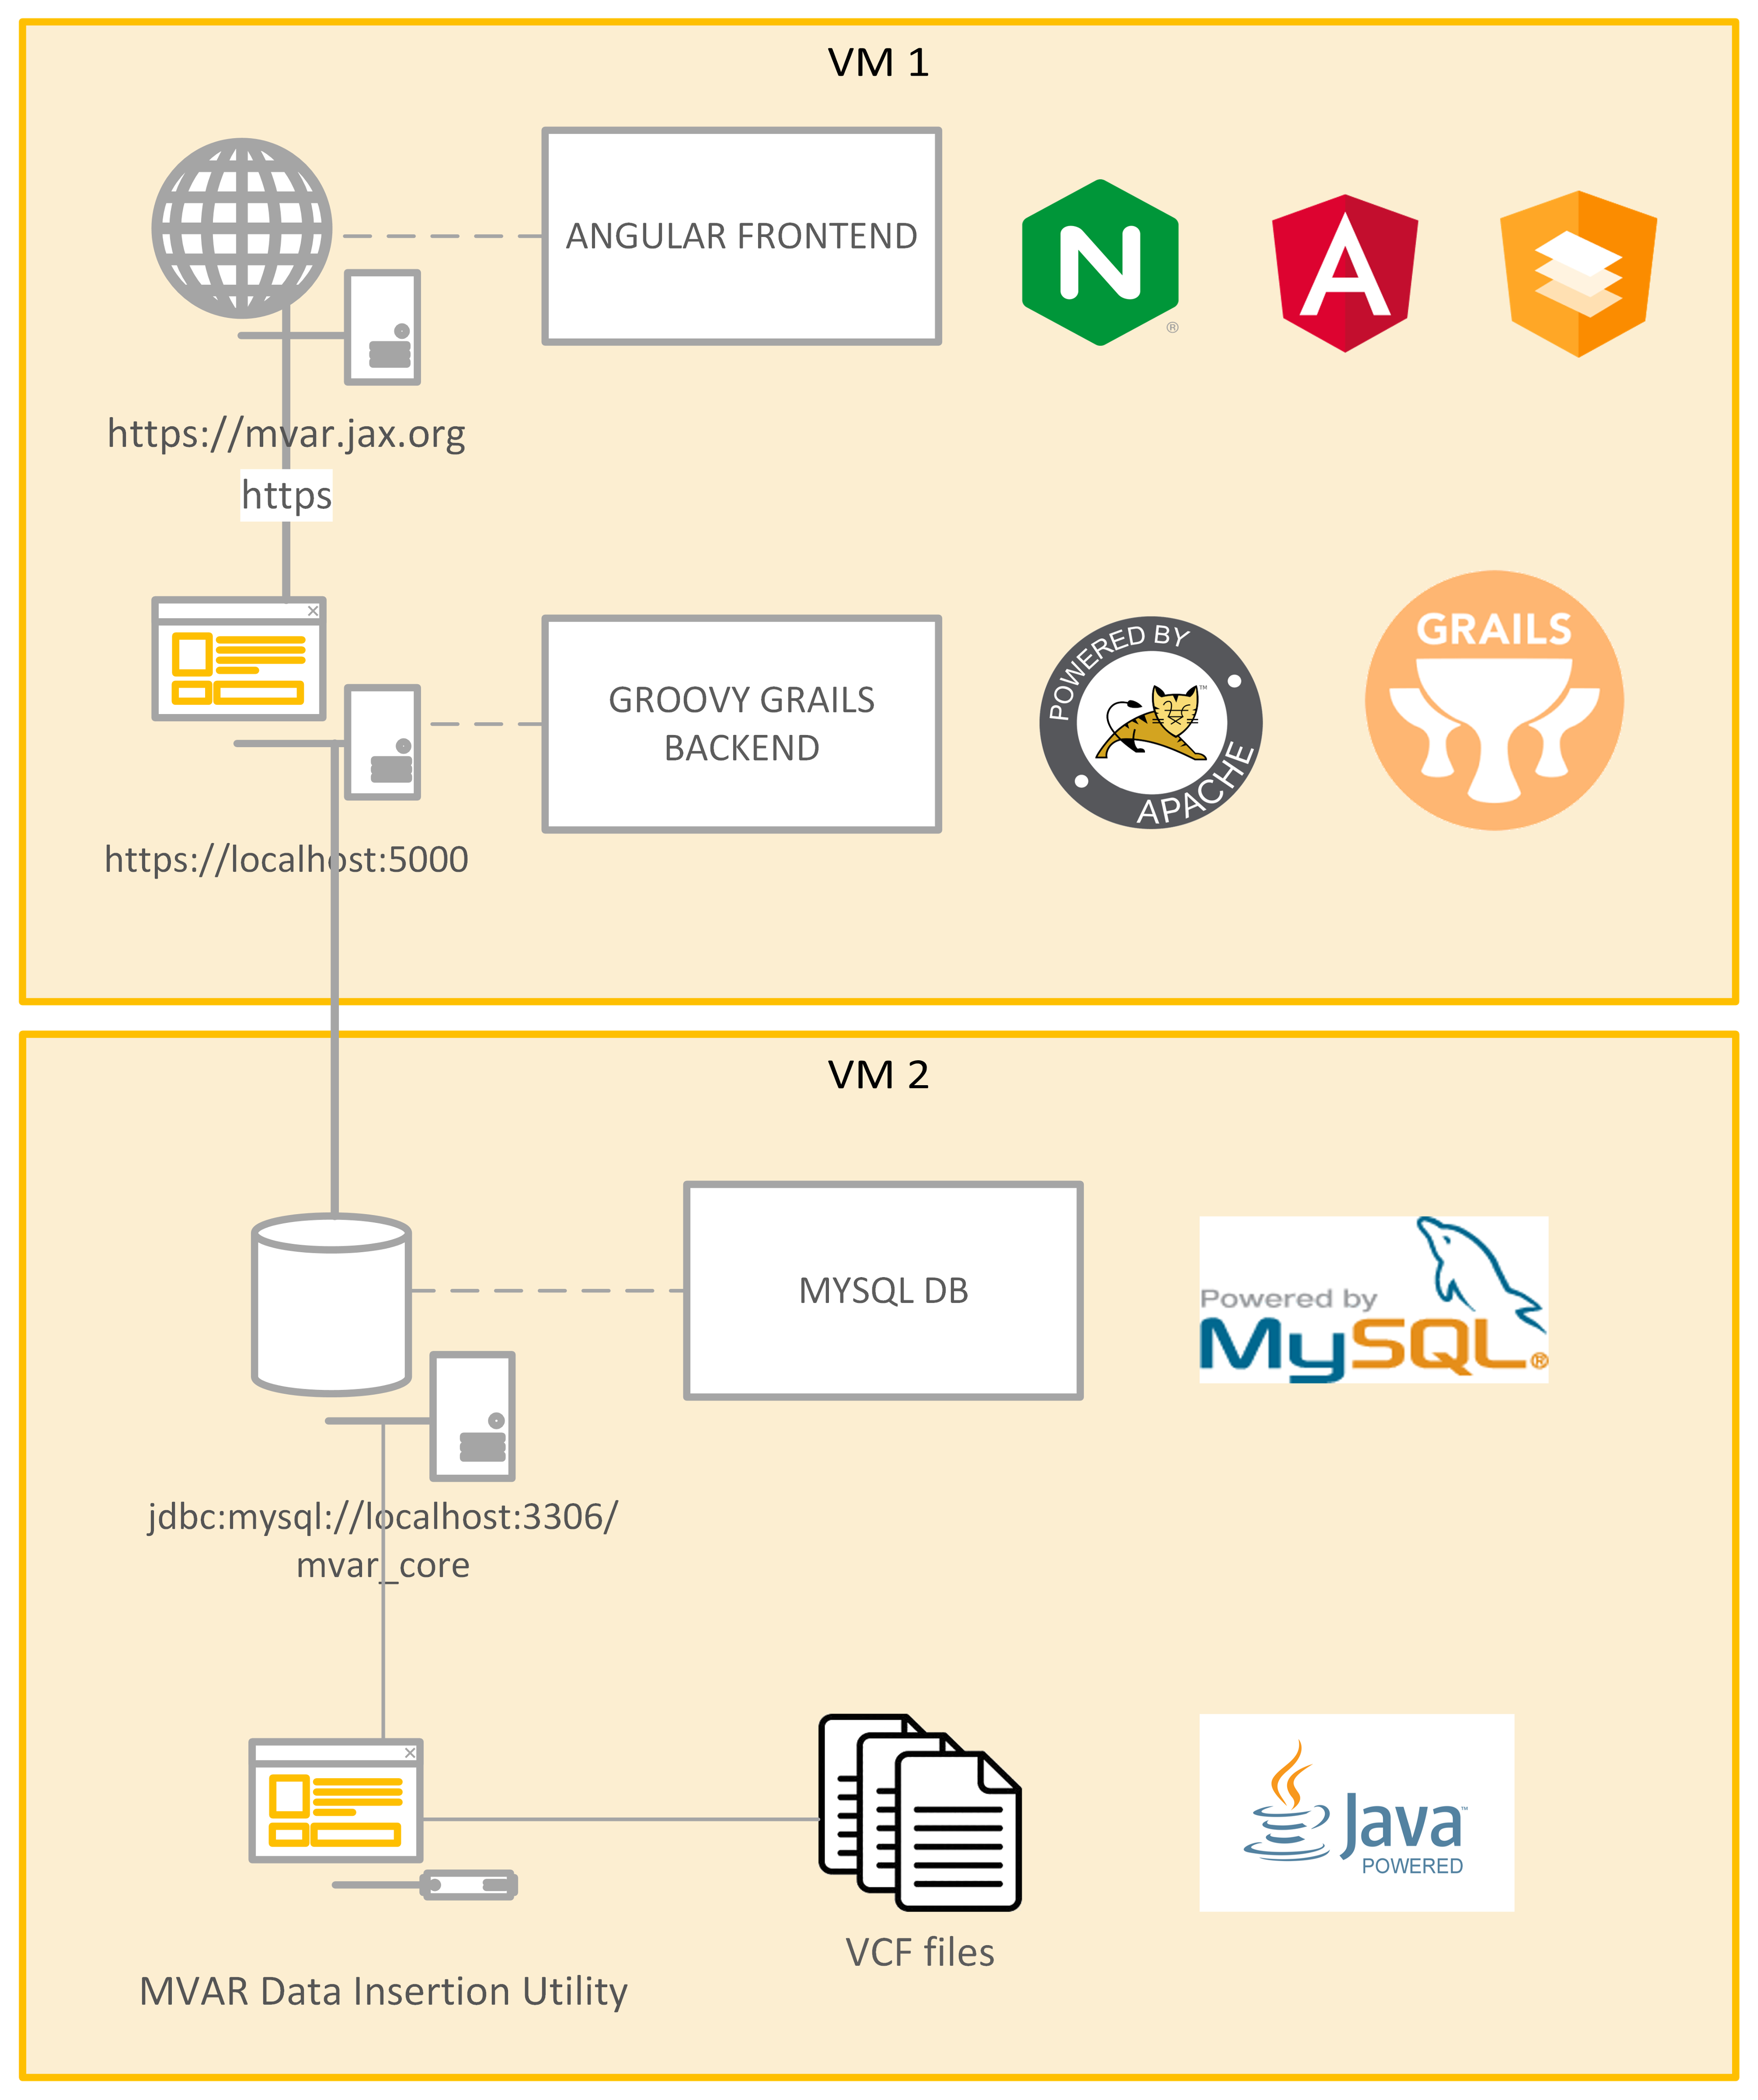
\includegraphics[width=0.5\linewidth]{server_architecture.png}
\caption{\label{fig:server_architecture}Server architecture and technologies}
\end{figure}

\section{MVAR User Interface and API}

MVAR supports programmatic data access to the registry through an Application Programming Interface (API) for interoperability. This API is used by a user-friendly web-application with rich user interfaces to query the database and display results (See Figures \ref{fig:search_result}, \ref{fig:variant_strain_distrib}). The API is also available to be a resource for other services or applications over HTTP with JSON data payloads. Wide-used industry frameworks like Angular and Groovy Grails were leveraged to build the MVAR web application.

\begin{figure}
\centering
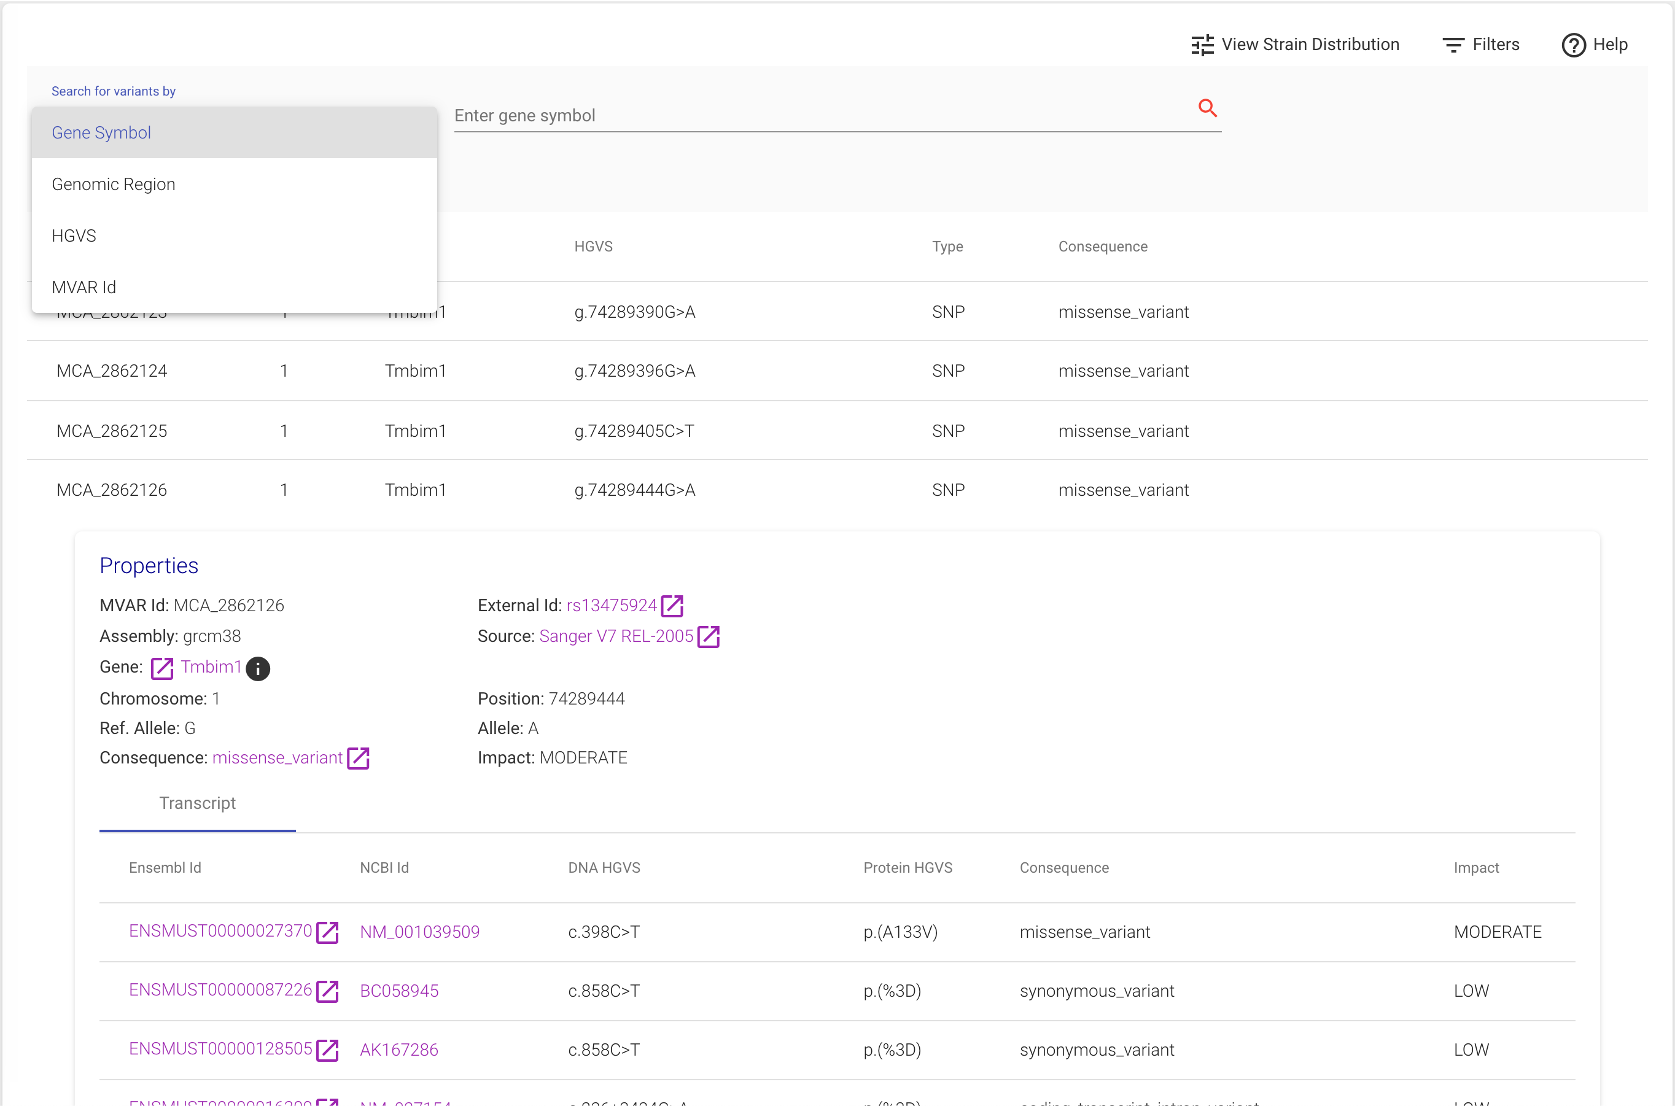
\includegraphics[width=0.9\linewidth]{search_result_ui.png}
\caption{\label{fig:search_result}Screenshot of a search result}
\end{figure}

\begin{figure}
\centering
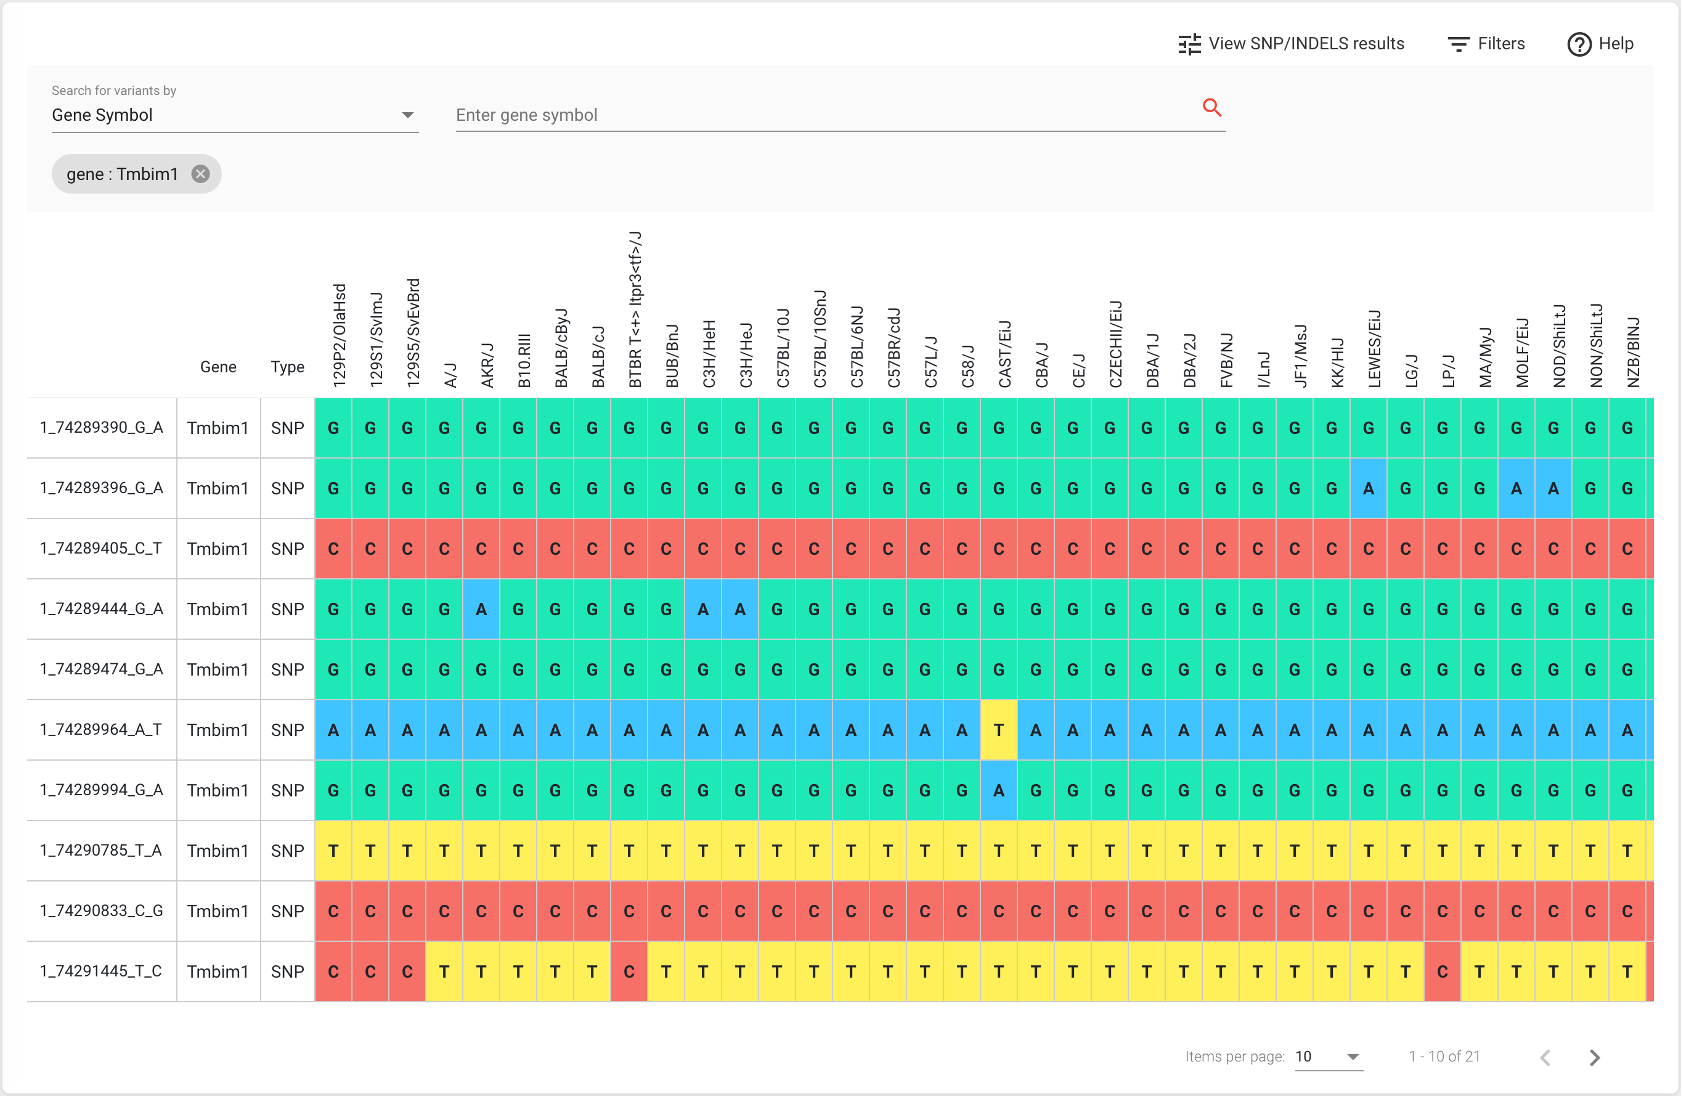
\includegraphics[width=0.9\linewidth]{variant_strain_distrib_ui.png}
\caption{\label{fig:variant_strain_distrib}Corresponding variant/strain distribution}
\end{figure}

\section{Main findings and biological relevance}

The MVAR integrates mouse genome variation data from multiple sources with functional and phenotypic annotations. Phenotype allele variants from MGI are converted into HGVS syntax to enable comparison to data from other genome variation resources. The data ingest pipeline for MVAR includes a canonicalization process to ensure genome variants are represented without redundancy and given unique persistent identifiers. Functional annotations for variants are made using Ensembl’s Variant Effect Predictor and Jannovar.

MVAR is maintained as a MySQL database accessed by a web-based application for variant search and display (\url{https://mvar.jax.org}). Users can search for variants by several criteria including gene name, genomic region, and HGVS notation. Results are displayed in both tabular and graphical formats. Programmatic data access to the registry through an Application Programming Interface (API) for interoperability. The API is also available to be a resource for other services or applications over HTTP with JSON data payloads. 
Significance. As an annotated genome variation resource for the laboratory mouse, MVAR is a unique resource for genotype-phenotype associations that leverages and integrates high-throughput SNP polymorphism data from the EVA, imputed SNP allele calls from GenomeMUSter \cite{ball23}, and phenotypic allele annotations from the MGI database.

\section{conclusion}

The lack of a comprehensive, annotated genome variation resource for mouse is a significant barrier to comparing variation and its biological consequences between mouse and human and limits the impact of many research and resource development programs within JAX. The MVAR project seeks to address this resource gap by bringing together investigators that have active projects in the area of genome variation in either mouse or human or both. Many of the investigators on this project have developed independent resources to curate or manage genome variation. This project aims to unify these efforts and build a common data resource. Future work will include the incorporation of structural variants into the MVAR registry.

\bibliographystyle{unsrt}
\bibliography{bibliography}

\end{document}